\documentclass[conference]{IEEEtran}
\IEEEoverridecommandlockouts

\usepackage{cite}
\usepackage{amsmath,amssymb,amsfonts}
\usepackage{algorithmic}
\usepackage{graphicx}
\usepackage{textcomp}
\usepackage{xcolor}
\usepackage{url}

\def\BibTeX{{\rm B\kern-.05em{\sc i\kern-.025em b}\kern-.08em
    T\kern-.1667em\lower.7ex\hbox{E}\kern-.125emX}}

\begin{document}

\title{Mainline-Disturbance-Aware Cooperative Gap Development for On-Ramp Merging}

\author{
\IEEEauthorblockN{First Author}
\IEEEauthorblockA{
\textit{Affiliation} \\
City, Country \\
email@example.com
}
}

\maketitle

\begin{abstract}
On-ramp merging with connected and automated vehicles is often formulated as
cooperative sequencing or trajectory planning, but a candidate gap may require
non-negligible mainline cooperation before it becomes safe. This paper proposes
a mainline-disturbance-aware cooperative gap development method for a local
single merging-vehicle (MV) decision. Candidate gaps are evaluated as
developable resources rather than static openings. For each gap, the available
forward and backward boundary-vehicle cooperation is bounded by adjacent-gap
safety margins, and a space-sensitive weighted quadratic adjustment estimates
the minimum necessary cooperation to satisfy the required merging gap. The
developed candidate is then scored by combining mainline cooperation cost and
MV ego merging cost, and the selected gap is converted into terminal time,
merging position, and a closed-form fifth-order feasible trajectory.
Experiments validate three aspects: the full chain selects an executable
developed gap in a representative case; ablation cases show no unnecessary
cooperation and adjustment allocation toward the boundary side with larger
residual margin; and representative successful-merging comparisons with a FIFO
cooperative baseline reduce affected mainline vehicles from 3--6 to 0--2,
lower mainline acceleration energy in all reported cases, and shorten recovery
time from 20.75--36.75~s to 0--13.10~s. These results support low-disturbance
local gap development rather than global traffic optimality.
\end{abstract}

\begin{IEEEkeywords}
On-ramp merging, connected and automated vehicles, cooperative gap development,
mainline disturbance, trajectory planning.
\end{IEEEkeywords}

\section{Introduction}
On-ramp merging is a typical conflict point where a ramp vehicle must enter a
mainline traffic stream while mainline vehicles attempt to preserve speed and
spacing. Connected and automated vehicles (CAVs) make it possible to coordinate
the merging vehicle (MV) and nearby mainline vehicles more actively than in
human-driven traffic. However, the essential question is not only whether the MV
can enter a gap. A safe merge may require the mainline traffic to create or
enlarge that gap, and this cooperation consumes boundary-vehicle motion,
neighboring spacing, and potentially the speed stability of following traffic.
Thus, mainline cooperation should not be treated as a free resource.

Cooperative merging and sequencing for CAVs have been widely studied. Surveys
and representative controllers have formulated the merging area as a coordinated
control zone, often assigning a passing order and optimizing vehicle motion to
improve safety, fuel use, or travel efficiency
\cite{riosTorres2017survey,riosTorres2017automated}. Further studies optimize
the merging sequence through game-theoretic or integrated sequence-trajectory
frameworks \cite{jing2019cooperative,chen2024integrated}. These approaches show
the value of coordination, but they typically regard mainline vehicles as
coordinated resources after the merging order or target interaction structure
has been specified. As a result, the local cost of developing each candidate gap
is not always the central object of valuation.

Trajectory-optimization methods provide another important line of work. They
can generate smooth, safe, or energy-efficient trajectories for automated
merging under speed, acceleration, collision-avoidance, and terminal constraints
\cite{ntousakis2016optimal,karimi2020cooperative}. Some recent formulations
also allow flexible merging positions or combine sequence generation with
trajectory planning \cite{tang2022hierarchical,chen2024integrated}. Such methods
are effective once a terminal gap, sequence, or interaction target is known, but
they do not by themselves answer how much bounded mainline cooperation is needed
to turn a spatially insufficient candidate gap into a safe merging gap.

Work on gap creation and gap development is closer to this issue. Earlier
reviews discussed intelligent-vehicle concepts for facilitating motorway
on-ramp merging \cite{scarinci2014control}, and state-constrained optimal
control has explicitly considered automated merging and gap development with
speed constraints \cite{zhou2018automated}. More recently, the congestion caused
by gap creation for ramp vehicles has been studied as a mainline-side effect
\cite{zhou2024congestion}. These studies indicate that facilitating vehicles can
pay a nontrivial cost when a gap is created. A remaining missing link is to
connect this observation to a compact candidate-gap evaluation chain: the
available cooperation of the boundary vehicles should be bounded by neighboring
gap safety margins, the required gap shortage should be allocated with minimum
disturbance, and the developed candidates should be compared through a joint
valuation of mainline cooperation and MV merging efficiency.

This paper reframes local on-ramp merging as a
mainline-disturbance-aware cooperative gap development problem. At a merging
decision instant, each candidate gap is treated as a developable traffic
resource rather than a static object selected only by its current length,
distance, or ego trajectory cost. For each candidate gap, the planner first
computes how much the front and rear boundary vehicles can safely contribute
without compressing adjacent gaps below a safety margin. It then estimates the
minimum necessary boundary-vehicle adjustment through a space-sensitive
quadratic cost. The resulting cooperation cost is combined with the MV ego cost
to select the best developed gap, which is finally converted into a merging
time, merging location, and feasible trajectory.

The main contributions are summarized as follows:
\begin{itemize}
    \item A mainline-disturbance-aware cooperative gap development formulation
    is introduced for on-ramp merging, where candidate gaps are evaluated by the
    bounded and costly cooperation required from their boundary vehicles rather
    than by static gap size alone.
    \item An adjacent-gap-preserving cooperation capacity model and a
    space-sensitive minimum-disturbance adjustment are developed to estimate the
    minimum necessary cooperation for each candidate gap under neighboring-gap
    safety margins.
    \item A disturbance-efficiency valuation and selected-gap execution chain
    are proposed to select the best developed gap and convert it into terminal
    time, terminal location, and a closed-form feasible MV trajectory.
\end{itemize}

The experiments are organized around three levels of evidence. First, a
feasibility case demonstrates the closed chain from candidate-gap evaluation to
selected developed-gap trajectory execution. Second, compact ablation cases
examine whether the proposed capacity and adjustment mechanisms allocate
cooperation according to neighboring-gap margins. Third, representative
successful-merging cases compare the proposed method with a fixed-order,
FIFO-style cooperative merging baseline based on Rios-Torres and Malikopoulos
\cite{riosTorres2017automated}. The external comparison focuses on mainline
disturbance reduction; the primary representative case additionally checks that
the disturbance reduction can be achieved with comparable physical merge timing.

\section{Problem Formulation}
Consider a local on-ramp merging decision at a planning instant. The target
mainline lane contains longitudinal vehicle positions
\(X=[x_1,\ldots,x_N]\), sorted in increasing order, and the merging vehicle
(MV) is located at \(x_m(0)\). Mainline vehicles are initially assumed to travel
at a reference speed \(v_{ref}\). The planner evaluates the candidate gaps
formed by adjacent target-lane vehicles. The \(i\)-th candidate gap is
\begin{equation}
    \mathrm{gap}_i=[x_{r,i},x_{f,i}],\quad
    G_i=x_{f,i}-x_{r,i},\quad
    c_i=\frac{x_{r,i}+x_{f,i}}{2},
    \label{eq:gap_definition}
\end{equation}
where \(x_{r,i}\) and \(x_{f,i}\) denote the rear and front boundary vehicles,
respectively, \(G_i\) is the current gap length, and \(c_i\) is the current
gap center.

Two safety lengths are distinguished. The required merging gap for inserting
the MV is
\begin{equation}
    G^{\mathrm{req}}=2D_h+l_m,
    \label{eq:required_gap}
\end{equation}
where \(D_h\) is the longitudinal safety headway and \(l_m\) is the MV length.
The adjacent-gap protection threshold is
\begin{equation}
    G^{\mathrm{adj}}=D_h+l_m.
    \label{eq:adjacent_gap}
\end{equation}
The former specifies the target gap size needed for a safe merge, while the
latter prevents boundary-vehicle cooperation from compressing neighboring
mainline gaps below a safety margin. Therefore, a candidate gap is not removed
only because \(G_i<G^{\mathrm{req}}\). Instead, its required shortage is
\begin{equation}
    \Delta_i=\max(0,G^{\mathrm{req}}-G_i).
    \label{eq:gap_shortage}
\end{equation}

The cooperation adjustment of candidate gap \(i\) is described by two
nonnegative quantities: \(\delta_{f,i}\), the forward displacement of the
front boundary vehicle, and \(\delta_{r,i}\), the backward displacement of the
rear boundary vehicle. These adjustments enlarge the target gap by
\(\delta_{f,i}+\delta_{r,i}\), but they also consume neighboring-gap margins
and thus are treated as bounded and costly mainline cooperation. The method
therefore estimates, for each candidate gap, a minimum necessary mainline
cooperation cost \(C_i^{\mathrm{coop}}\) and an MV ego merging cost
\(C_i^{\mathrm{ego}}\). The selected developed gap minimizes the integrated
valuation
\begin{equation}
    J_i=w_c C_i^{\mathrm{coop}}+w_e C_i^{\mathrm{ego}},
    \label{eq:abstract_score}
\end{equation}
subject to gap safety, neighboring-gap capacity, and MV kinematic constraints,
including
\begin{equation}
    v_{\min}\leq v_m(t)\leq v_{\max},\qquad
    a_{\min}\leq a_m(t)\leq a_{\max}.
\end{equation}

This formulation focuses on a single MV at one merging decision instant. The
target-lane positions are assumed to be available from perception,
communication, or the experimental scenario, and the boundary vehicles of a
candidate gap are assumed to be cooperative CAVs. A basic kinematic reachability
check may be applied before valuation to avoid physically unreachable gaps, but
reachability is only a screening condition in this paper. Multi-MV rolling
coordination, stochastic traffic generation, mixed CAV/HDV response, lane-change
gap supply, and closed-loop traffic simulation are outside the scope of the
present ICUS formulation.

\section{Mainline-Disturbance-Aware Cooperative Gap Development}
The proposed planner decomposes the local problem into four steps. First, it
computes how much each boundary vehicle can safely contribute while preserving
adjacent gaps. Second, it estimates the minimum necessary adjustment for each
candidate gap through a space-sensitive convex problem. Third, it scores all
developed candidates by combining mainline cooperation cost and MV ego cost.
Finally, it executes only the selected developed gap by generating the boundary
adjustment and the MV trajectory.

\subsection{Adjacent-Gap-Preserving Cooperation Capacity}
For an interior candidate gap \(\mathrm{gap}_i=[x_i,x_{i+1}]\), the adjacent
mainline gaps are \(G_{i-1}=x_i-x_{i-1}\) and
\(G_{i+1}=x_{i+2}-x_{i+1}\). When the front boundary vehicle moves forward, it
compresses the front-side neighboring gap. When the rear boundary vehicle moves
backward, it compresses the rear-side neighboring gap. Hence, the maximum safe
cooperation capacities are defined as
\begin{equation}
    \bar{\delta}_{f,i}=\max(0,G_{i+1}-G^{\mathrm{adj}}),
    \qquad
    \bar{\delta}_{r,i}=\max(0,G_{i-1}-G^{\mathrm{adj}}).
    \label{eq:capacity}
\end{equation}
These bounds are state-dependent: a boundary vehicle can contribute more only
when the adjacent gap on its outside has sufficient residual margin.

Candidate gap \(i\) can be developed into a safe merging gap by longitudinal
boundary-vehicle cooperation only if
\begin{equation}
    \bar{\delta}_{f,i}+\bar{\delta}_{r,i}\geq \Delta_i.
    \label{eq:coop_feasibility}
\end{equation}
The cooperatively developable set is then
\begin{equation}
    \mathcal{G}_{\mathrm{coop}}
    =
    \left\{
    i\,\middle|\,
    \bar{\delta}_{f,i}+\bar{\delta}_{r,i}\geq \Delta_i
    \right\}.
    \label{eq:coop_set}
\end{equation}
If \(\Delta_i=0\), the current gap already satisfies the required merging
length and the minimum cooperation estimate is
\(\delta_{f,i}^*=\delta_{r,i}^*=0\).

\subsection{Space-Sensitive Minimum-Disturbance Adjustment}
For a developable candidate gap with \(\Delta_i>0\), the shortage should be
allocated to the two boundary vehicles with minimum mainline disturbance. The
space-sensitive weights are
\begin{equation}
    \gamma_{f,i}
    =
    \left(\frac{\delta_{ref}}{\bar{\delta}_{f,i}}\right)^q,
    \qquad
    \gamma_{r,i}
    =
    \left(\frac{\delta_{ref}}{\bar{\delta}_{r,i}}\right)^q,
    \label{eq:gamma}
\end{equation}
for positive capacities. A smaller residual neighboring-gap margin leads to a
larger weight, so the optimization naturally avoids consuming the tighter side.
The candidate-level cooperation estimate is obtained from
\begin{align}
    \min_{\delta_{f,i},\delta_{r,i}}\quad
    C_i^{\mathrm{coop}}
    &=
    \gamma_{f,i}\delta_{f,i}^2+
    \gamma_{r,i}\delta_{r,i}^2
    \label{eq:coop_qp}\\
    \mathrm{s.t.}\quad
    \delta_{f,i}+\delta_{r,i}&\geq \Delta_i, \notag\\
    0\leq \delta_{f,i}&\leq \bar{\delta}_{f,i}, \notag\\
    0\leq \delta_{r,i}&\leq \bar{\delta}_{r,i}. \notag
\end{align}
Because the objective increases with the adjustment magnitudes, the optimum
satisfies \(\delta_{f,i}+\delta_{r,i}=\Delta_i\). Thus, the two-dimensional
problem admits a one-dimensional projected solution. Define
\begin{equation}
    L_i=\max(0,\Delta_i-\bar{\delta}_{r,i}),\qquad
    U_i=\min(\bar{\delta}_{f,i},\Delta_i),
    \label{eq:projection_bounds}
\end{equation}
and the unconstrained weighted split
\begin{equation}
    \delta_{f,i}^{\mathrm{raw}}
    =
    \frac{\gamma_{r,i}}{\gamma_{f,i}+\gamma_{r,i}}\Delta_i.
    \label{eq:raw_split}
\end{equation}
With \(\Pi_{[L_i,U_i]}(\cdot)\) denoting projection onto
\([L_i,U_i]\), the closed-form estimate is
\begin{equation}
    \delta_{f,i}^*
    =
    \Pi_{[L_i,U_i]}(\delta_{f,i}^{\mathrm{raw}}),
    \qquad
    \delta_{r,i}^*
    =
    \Delta_i-\delta_{f,i}^*.
    \label{eq:projected_solution}
\end{equation}
These quantities are candidate-level estimates used for valuation; no physical
adjustment is applied before the best developed gap is selected.

\subsection{Disturbance-Efficiency Valuation for Developed Gaps}
The adjustment estimate shifts the center of the developed candidate gap by
\begin{equation}
    \Delta c_i=\frac{\delta_{f,i}^*-\delta_{r,i}^*}{2}.
    \label{eq:center_shift}
\end{equation}
Consequently, the MV must match the terminal displacement
\begin{equation}
    d_i=c_i+\frac{\delta_{f,i}^*-\delta_{r,i}^*}{2}-x_m(0).
    \label{eq:terminal_displacement}
\end{equation}
If the front boundary contributes more, the developed gap center moves forward;
if the rear boundary contributes more, the developed gap center moves backward.
This center shift links mainline cooperation to the MV ego trajectory cost.

For each developed candidate, the cooperation cost is
\begin{equation}
    C_i^{\mathrm{coop}}
    =
    \gamma_{f,i}(\delta_{f,i}^*)^2+
    \gamma_{r,i}(\delta_{r,i}^*)^2.
    \label{eq:coop_cost}
\end{equation}
Using the terminal time rule in the next subsection, the MV ego cost is
\begin{equation}
    C_i^{\mathrm{ego}}
    =
    \frac{K d_i^2}{(t_{m,i}^*)^3}
    +
    w_t t_{m,i}^*,
    \qquad
    K=\frac{120}{7}.
    \label{eq:ego_cost}
\end{equation}
The disturbance-efficiency score is
\begin{equation}
    J_i
    =
    w_c C_i^{\mathrm{coop}}
    +
    w_e C_i^{\mathrm{ego}}.
    \label{eq:valuation}
\end{equation}
The best developed gap is selected by
\begin{equation}
    i^*
    =
    \underset{i\in\mathcal{G}_{\mathrm{coop}}}{\arg\min}\;J_i.
    \label{eq:selected_gap}
\end{equation}
The order is important: all candidates are first estimated and scored, then
\(i^*\) is selected, and only the selected gap is executed.

\subsection{Terminal Time, Merging Location, and Feasible Trajectory}
The candidate terminal time is computed from a fifth-order smooth transition
\begin{equation}
    S(\tau)=10\tau^3-15\tau^4+6\tau^5,\qquad
    \tau=\frac{t}{t_m},
    \label{eq:smooth_function}
\end{equation}
which satisfies zero relative velocity and acceleration at both ends. The
unconstrained energy-time tradeoff gives
\begin{equation}
    t_{m,i}^{0}
    =
    \left(\frac{3K d_i^2}{w_t}\right)^{1/4}.
    \label{eq:t_unconstrained}
\end{equation}
Let \(a_{\lim}=\min(a_{\max},|a_{\min}|)\). Since
\(\max_{\tau\in[0,1]}|S''(\tau)|=10/\sqrt{3}\), the acceleration constraint
requires
\begin{equation}
    t_{a,i}
    =
    \sqrt{
    \frac{\frac{10}{\sqrt{3}}|d_i|}{a_{\lim}}
    }.
    \label{eq:t_acc}
\end{equation}
The velocity constraint uses \(S'_{\max}=1.875\), yielding
\begin{equation}
    t_{v,i}
    =
    \begin{cases}
    \dfrac{1.875|d_i|}{v_{\max}-v_{ref}}, & d_i\geq 0,\\[8pt]
    \dfrac{1.875|d_i|}{v_{ref}-v_{\min}}, & d_i<0.
    \end{cases}
    \label{eq:t_vel}
\end{equation}
The final candidate terminal time and merging location are
\begin{equation}
    t_{m,i}^*
    =
    \max(t_{m,i}^{0},t_{a,i},t_{v,i}),
    \qquad
    p_{m,i}=x_m(0)+v_{ref}t_{m,i}^*+d_i.
    \label{eq:terminal_time_location}
\end{equation}

After \(i^*\) is selected, define
\begin{align}
    d^*&=d_{i^*},&
    t_m^*&=t_{m,i^*}^*,&
    p_m^*&=p_{m,i^*}, \notag\\
    \delta_f^*&=\delta_{f,i^*}^*,&
    \delta_r^*&=\delta_{r,i^*}^*. \label{eq:selected_quantities}
\end{align}
For \(0\leq t\leq t_m^*\), the MV trajectory is
\begin{align}
    x_m(t)
    &=
    x_m(0)+v_{ref}t+
    d^*S\left(\frac{t}{t_m^*}\right), \label{eq:mv_position}\\
    v_m(t)
    &=
    v_{ref}
    +
    \frac{d^*}{t_m^*}
    S'\left(\frac{t}{t_m^*}\right), \label{eq:mv_velocity}\\
    a_m(t)
    &=
    \frac{d^*}{(t_m^*)^2}
    S''\left(\frac{t}{t_m^*}\right). \label{eq:mv_acc}
\end{align}
The selected rear and front boundary vehicles follow
\begin{align}
    x_r(t)
    &=
    x_r^*+v_{ref}t-
    \delta_r^*S\left(\frac{t}{t_m^*}\right), \label{eq:rear_traj}\\
    x_f(t)
    &=
    x_f^*+v_{ref}t+
    \delta_f^*S\left(\frac{t}{t_m^*}\right), \label{eq:front_traj}
\end{align}
where \(x_r^*=x_{r,i^*}\) and \(x_f^*=x_{f,i^*}\). Therefore, the selected
gap length evolves as
\begin{equation}
    G^*(t)
    =
    G_{i^*}
    +
    (\delta_f^*+\delta_r^*)
    S\left(\frac{t}{t_m^*}\right),
    \label{eq:dynamic_gap}
\end{equation}
and at the terminal time
\begin{equation}
    G^*(t_m^*)=G_{i^*}+\delta_f^*+\delta_r^*
    \geq G^{\mathrm{req}}.
    \label{eq:terminal_gap}
\end{equation}
The developed gap center is
\begin{equation}
    c^*(t)
    =
    c_{i^*}+v_{ref}t+
    \frac{\delta_f^*-\delta_r^*}{2}
    S\left(\frac{t}{t_m^*}\right),
    \label{eq:dynamic_center}
\end{equation}
so \(c^*(t_m^*)=p_m^*\). Thus, the selected developed gap is converted into a
terminal time, terminal position, and feasible MV trajectory while maintaining
the required developed gap length.

\section{Experiments}
The experiments are designed to verify the proposed chain at three levels:
candidate-gap feasibility, capacity-and-adjustment behavior, and external
mainline disturbance relative to a FIFO baseline. All experiments use local
single-MV merging configurations with the target-lane vehicles initially moving
at \(v_{ref}=20~\mathrm{m/s}\). The safety parameters give
\(G^{\mathrm{req}}=85~\mathrm{m}\) and
\(G^{\mathrm{adj}}=45~\mathrm{m}\). The valuation weights are fixed as
\(w_c=0.2\), \(w_e=1\), and \(w_t=10\) across all cases.

\subsection{Experimental Setup}
The proposed method, denoted as Proposed in the tables, evaluates all candidate
mainline gaps, estimates the minimum necessary boundary-vehicle adjustment,
selects the best developed gap according to \(J_i\), and then executes only the
selected gap. The external baseline is a FIFO cooperative merging controller
that organizes vehicles through a fixed-order and fixed-spacing rule. In the
baseline logs, the physical merge-entry and merge-exit locations are
\(x=555~\mathrm{m}\) and \(x=600~\mathrm{m}\), respectively. These locations
are used to confirm that both methods complete the physical merge, but they are
not used as the main performance metrics because the two methods optimize
different objectives.

The internal validation uses the quantities introduced in Sections II and III:
\(\Delta_i\), \(\bar{\delta}_{f,i}/\bar{\delta}_{r,i}\),
\(\delta_{f,i}^*/\delta_{r,i}^*\), \(C_i^{\mathrm{coop}}\),
\(C_i^{\mathrm{ego}}\), and \(J_i\). The external comparison focuses on
mainline disturbance: the number of affected mainline vehicles, mainline
acceleration energy, and recovery time. Merge-point and spacing quantities are
reported only as planning context because the FIFO baseline enforces a fixed
merge-entry location and a fixed target spacing.

\subsection{Feasibility Validation}
The first experiment verifies that candidate-gap evaluation can be converted
into an executable merge trajectory. The representative configuration uses
\[
    X=[-180,-90,-25,30,110,190,250]~\mathrm{m}.
\]
Table~\ref{tab:feasibility_eval} lists all candidate gaps. The selected row is
not the largest current gap or the ego-only nearest option. Instead, gap 4 is
selected because its small shortage can be developed by a local front-boundary
adjustment while keeping the combined disturbance-efficiency score lower than
the other candidates.

\begin{table}[t]
\caption{Candidate-Gap Evaluation and Selection}
\label{tab:feasibility_eval}
\centering
\scriptsize
\resizebox{\columnwidth}{!}{%
\begin{tabular}{c c c c c c c c c}
\hline
Gap & Interval (m) & \(G_i\) & \(\Delta_i\) & Cap. f/r & Adj. f/r & \(C_i^{\mathrm{coop}}\) & \(C_i^{\mathrm{ego}}\) & \(J_i\) \\
\hline
1 & \([-180,-90]\) & 90 & 0 & 20/100 & 0/0 & 0.00 & 233.30 & 233.30 \\
2 & \([-90,-25]\) & 65 & 20 & 10/45 & 0/20 & 88.55 & 164.96 & 182.68 \\
3 & \([-25,30]\) & 55 & 30 & 35/20 & 28.99/1.01 & 869.72 & 81.54 & 255.48 \\
\textbf{4} & \(\mathbf{[30,110]}\) & \textbf{80} & \textbf{5} & \textbf{35/10} & \textbf{5/0} & \textbf{25.00} & \textbf{171.81} & \textbf{176.81} \\
5 & \([110,190]\) & 80 & 5 & 15/35 & 0/5 & 25.00 & 294.19 & 299.19 \\
6 & \([190,250]\) & 60 & -- & -- & -- & -- & -- & infeasible \\
\hline
\end{tabular}%
}
\end{table}

For the selected developed gap, the estimated terminal quantities are
\(d^*=72.5~\mathrm{m}\), \(t_m^*=13.594~\mathrm{s}\), and
\(p_m^*=344.375~\mathrm{m}\). Fig.~\ref{fig:feasibility_traj} shows the
resulting time-space trajectory. The MV reaches the developed gap center at the
terminal time, while only the selected boundary vehicle is adjusted. This
validates the closed chain from candidate-level estimation to selected-gap
execution.

\begin{figure}[t]
\centering
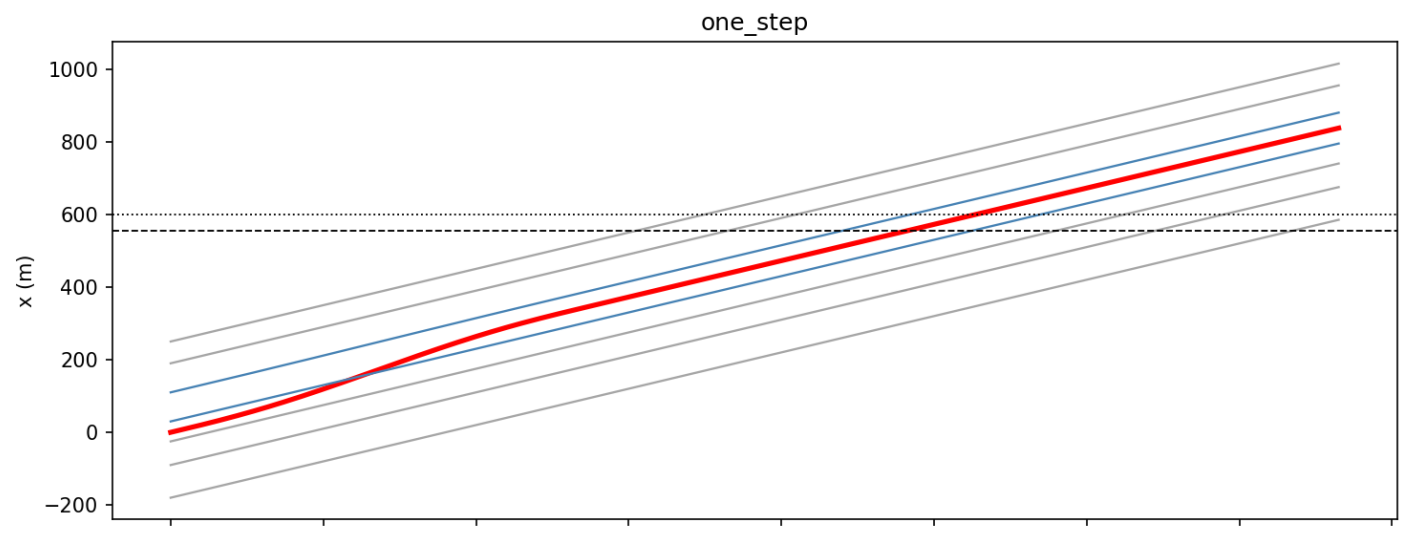
\includegraphics[width=\linewidth]{figures/feasibility_trajectory.png}
\caption{Feasibility trajectory generated for the selected developed gap. The
red curve denotes the MV trajectory, blue curves denote the selected boundary
vehicles, and gray curves denote non-selected mainline vehicles.}
\label{fig:feasibility_traj}
\end{figure}

\subsection{Capacity and Adjustment Ablation}
The second experiment checks whether the adjacent-gap capacity and
space-sensitive adjustment behave as intended. Four representative cases are
constructed from the same evidence package. Table~\ref{tab:capacity_ablation}
compares an equal split with the proposed weighted adjustment. The purpose is
not to claim a global traffic optimum, but to verify the mechanism: no
unnecessary cooperation is introduced when \(\Delta_i=0\), symmetric margins
lead to symmetric adjustment, and asymmetric margins shift the adjustment burden
toward the side with more residual neighboring space.

\begin{table}[t]
\caption{Capacity and Adjustment Ablation}
\label{tab:capacity_ablation}
\centering
\scriptsize
\resizebox{\columnwidth}{!}{%
\begin{tabular}{c c c c c c c}
\hline
Case & Selected gap (m) & \(\Delta_i\) & Cap. f/r & Equal f/r & Proposed f/r & Verified behavior \\
\hline
C1 & \([10,95]\) & 0 & 30/100 & 0/0 & 0/0 & no unnecessary cooperation \\
C2 & \([-20,45]\) & 20 & 35/35 & 10/10 & 10/10 & symmetric allocation \\
C3 & \([30,110]\) & 5 & 35/10 & 2.5/2.5 & 5/0 & front-side larger margin \\
C4 & \([-20,60]\) & 5 & 10/35 & 2.5/2.5 & 0/5 & rear-side larger margin \\
\hline
\end{tabular}%
}
\end{table}

The last two rows illustrate the role of the space-sensitive weights in
(\ref{eq:gamma}). With a larger front-side capacity, the proposed solution moves
the front boundary vehicle and avoids consuming the tighter rear-side margin.
With a larger rear-side capacity, the adjustment is shifted to the rear
boundary vehicle. Thus, the compact ablation validates the intended
capacity-preserving behavior of the adjustment model.

\subsection{Representative External Comparison with FIFO Baseline}
The third experiment compares the proposed method with the FIFO baseline in
five representative successful-merging cases. A key distinction is that the FIFO
baseline is designed to organize vehicles according to a fixed order and a
fixed target spacing. It may therefore accelerate or decelerate multiple
mainline vehicles to form the prescribed spacing pattern. For this reason,
entry time, exit time, minimum spacing, and minimum TTC are not used as the main
cross-method comparison metrics in this section. The comparison instead asks
whether successful merging can be achieved with less mainline cooperation.

Table~\ref{tab:external_disturbance} shows the disturbance metrics. Across all
five cases, the proposed method affects fewer mainline vehicles than the FIFO
baseline. In Cases B and C, the selected developed gap requires no mainline
adjustment, while FIFO still adjusts multiple mainline vehicles to satisfy its
queue-spacing rule. In Cases A and E, the proposed method confines the
cooperation to one boundary vehicle. Case D is the most demanding case for the
proposed method, but it still reduces the affected mainline vehicles from five
to two and shortens the recovery time from \(26.25~\mathrm{s}\) to
\(5.30~\mathrm{s}\).

\begin{table}[t]
\caption{External Comparison on Mainline Disturbance}
\label{tab:external_disturbance}
\centering
\scriptsize
\resizebox{\columnwidth}{!}{%
\begin{tabular}{c c c c c}
\hline
Case & Method & Affected veh. & Acc. energy & Recovery time (s) \\
\hline
A & Proposed & 1 & 0.171 & 13.10 \\
A & FIFO & 6 & 22.188 & 31.00 \\
B & Proposed & 0 & 0.000 & 0.00 \\
B & FIFO & 4 & 52.652 & 20.75 \\
C & Proposed & 0 & 0.000 & 0.00 \\
C & FIFO & 3 & 2.744 & 36.75 \\
D & Proposed & 2 & 22.715 & 5.30 \\
D & FIFO & 5 & 67.262 & 26.25 \\
E & Proposed & 1 & 1.714 & 6.20 \\
E & FIFO & 5 & 31.662 & 27.50 \\
\hline
\end{tabular}%
}
\end{table}

Fig.~\ref{fig:external_time_space} visualizes one representative comparison.
The proposed method develops and executes a local selected gap, whereas the
FIFO baseline reorganizes a broader set of mainline vehicles according to its
fixed-spacing logic. This figure is used to illustrate the difference in
control mechanism rather than to compare physical entry or exit timing.

\begin{figure}[t]
\centering
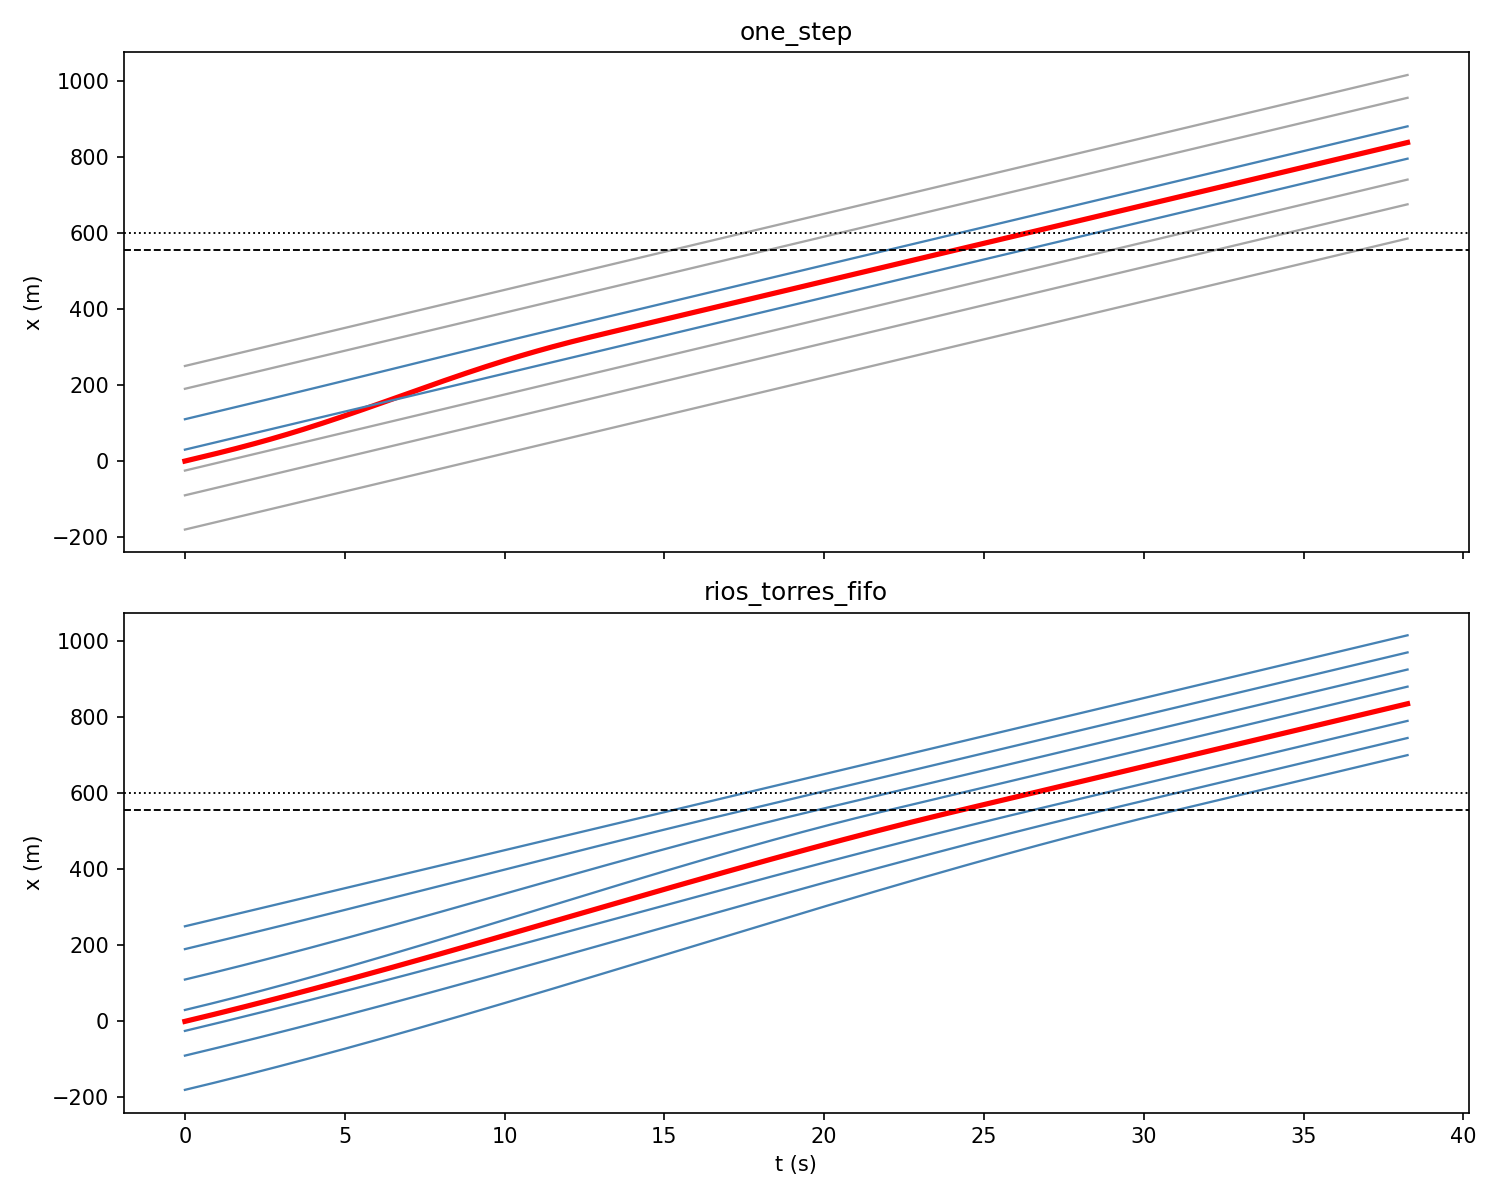
\includegraphics[width=\linewidth]{figures/external_time_space_comparison.png}
\caption{Representative time-space comparison between the proposed method and
the FIFO baseline. The red curve denotes the MV, and the mainline trajectories
show that FIFO regulates a broader vehicle set to form its fixed-spacing queue.}
\label{fig:external_time_space}
\end{figure}

Table~\ref{tab:merge_context} gives the corresponding planning context. The
proposed method computes a selected-gap merging location from the developed gap,
whereas the FIFO baseline uses the fixed physical merge-entry location in this
experiment package. Similarly, the proposed method reports the resulting
minimum spacing after selected-gap execution, while the FIFO value reflects its
fixed spacing target. These quantities support the safety-feasibility
interpretation, but they are not mixed with the disturbance metrics in
Table~\ref{tab:external_disturbance}.

\begin{table}[t]
\caption{Merge-Placement and Spacing Context}
\label{tab:merge_context}
\centering
\scriptsize
\resizebox{\columnwidth}{!}{%
\begin{tabular}{c c c c}
\hline
Method & Merge-location treatment & Min. spacing treatment & Role \\
\hline
Proposed & computed \(p_m\) from selected gap, \(118.98\)--\(344.38~\mathrm{m}\) & observed \(55\)--\(85~\mathrm{m}\) & planning context \\
FIFO & fixed physical entry, \(555~\mathrm{m}\) & fixed \(45~\mathrm{m}\) target & baseline setting \\
\hline
\end{tabular}%
}
\end{table}

Overall, the external comparison supports a narrow claim: in representative
successful-merging cases, evaluating developed gaps by the proposed
disturbance-efficiency score can substantially reduce the range, intensity, and
duration of mainline cooperation. The results do not imply that the method is
an always-fastest merging controller or a global traffic optimizer.

\section{Conclusion}
This paper presented a mainline-disturbance-aware cooperative gap development
method for local on-ramp merging. The central idea is that a candidate gap is
not only selected from the current mainline traffic state, but can be developed
through bounded and costly cooperation from its boundary vehicles. The proposed
formulation first constrains boundary-vehicle contributions by adjacent-gap
safety margins, then estimates the minimum necessary cooperation through a
space-sensitive weighted quadratic adjustment, and finally selects the best
developed gap by a disturbance-efficiency valuation. The selected gap is further
converted into a merging time, merging location, and feasible fifth-order MV
trajectory.

The experiments support this chain at three levels. The feasibility case shows
that candidate-gap evaluation can be closed into selected-gap trajectory
execution. The capacity and adjustment ablation verifies that the method avoids
unnecessary cooperation and shifts the adjustment burden toward the side with
larger neighboring-gap margin. Representative comparisons with a FIFO
cooperative merging baseline further show that the proposed method can reduce
the number of affected mainline vehicles, mainline acceleration energy, and
recovery time in successful-merging cases. These findings support the proposed
method as a lightweight and interpretable local gap-development planner. Future
work will extend the local longitudinal gap-development model to denser and
mixed traffic conditions with rolling coordination and closed-loop simulation.

\section*{Acknowledgment}
If you do not need acknowledgments or funding information, you can delete this
section before submission.

\bibliographystyle{IEEEtran}
\bibliography{refs}

\end{document}
